% !TEX root = ../arbeit.tex
\chapter{Interviews}\label{chapter:interview}
First of all, the user requirements for a \acf{PROCAMS} had to be determined. Therefore, structured interviews were conducted, to figure out how such a system could be employed in a domestic environment and would be used by end users. In interviews potential end users could remark their ideas and possible application scenarios. From the obtained information possible use-cases as well as the hardware and software requirements for a PROCAMS were derived. In the following the realised interviews are described and their results are discussed.


\section{Methodology}
For explaining the typical properties and abilities of a PROCAMS and for stimulating the creativity of the participants, a simple mock-up was built (see \autoref{img:mockup}). It comprises a portable battery powered LED projector PocketCinema V60 by AIPTEK contained in a cardboard box. The projector provides \SI{50}{ANSI} Lumen and projects images up to \SI{152}{\cm} in diagonal size. On the left side, it has a continuous rotating wheel to focus the projection. On the cardboard box, several hardware components are illustrated. On the front, a depth sensing camera loosely based on a PrimeSense carmine is shown. On the left side, a LCD display with some information and beneath four buttons (select, up, down, back) are affixed. On the backside, a big power button is illustrated. The mock-up has a total size of \SI{12.5x6.5x6}{\cm} and weighs \SI{195}{\g}. It is mounted on a tripod with flexible, wrappable legs which allows the user to place or attach it almost anywhere.

The interviews took place in the participant's home. To create a relaxed atmosphere and enable innocuous speaking no audio recording was made. Notes and ideas were drafted down on a clipboard. At the beginning of an interview session some introductory words about ubiquitous computing and what the following interview is all about were narrated. 
\begin{figure}[htbp]
\begin{center}
\includegraphics[width=0.5\textwidth]{images/interview/mockup_nobg.png}
\caption{Simple mock-up for interviews}
\label{img:mockup}
\end{center}
\end{figure}

The structured interviews were separated into three parts. First, every room of the participants home was inspected. They were called upon several questions about how they would use the \ac{PROCAMS}. In particular, how they would place or mount the system, which were the typical projection surfaces, how they would interact and what content they would like to project. Furthermore, they were asked to build a potential setup with the provided mock-up. There were several pre-designed non interactive widget examples stored on the projector. Widgets are small graphical items which present a specific content to the user. Some of them are illustrated in Figure \ref{img:mockupContent}.
Widgets were displayed when the participant referred to a suitable one and a realistic setup with the projected widget was constructed.
Then different interaction methods were discussed. To avoid biasing the results and ideas of the participant pre-designed widgets were not presented beforehand.

\begin{figure}[htbp]
        \centering
        \begin{subfigure}[b]{0.3\textwidth}
                \includegraphics[width=\textwidth]{images/interview/samples/clock.png}
                \caption{Clock widget}
                \label{img:cooking1}
        \end{subfigure}%
         \hfill 
        \begin{subfigure}[b]{0.3\textwidth}
                \includegraphics[width=\textwidth]{images/interview/samples/facebook.png}
                \caption{Facebook widget}
                \label{img:cooking1}
        \end{subfigure}
         \hfill
        \begin{subfigure}[b]{0.3\textwidth}
                \includegraphics[width=\textwidth]{images/interview/samples/weather.png}
                \caption{Weather widget}
                \label{fig:mouse}
        \end{subfigure}
        \caption{Pre-designed content}\label{img:mockupContent}
\end{figure}

The second part was a short questionnaire about the general requirements for a \ac{PROCAMS}. This part aimed to summarise the basic hardware requirements and design decisions. For example if a separate screen, like illustrated at the mock-up, would be necessary or if the \ac{PROCAMS} should be movable. Both, outcome of the interview and the questionnaire are discussed in detail in~\autoref{sec:interfacesINT}.

The last part of the interview was a questionnaire which asked for demographic data and technical understanding of the participant as well as the size of the living area and the housing situation. These results are written down in the next section. The whole interview including the questionnaire took 56 minutes on average.

			
\section{Participants and Environment}
Interviews were taken in a time period of three weeks. Eighteen participants, half male and half female, took part in the interviews. Their age ranged between 22 and 58 with an average age of 29.5.  Half of the participants were students with a technical background. The remaining were students of other fields (22\%) or employed. Looking at the technical affinity, 15 of the participants used a smart phone for more than two years. Only one-third of them already had been used a larger touch device, like a touch table or touch notebook. More than half of participants (61\%) had experience with free-space gestures interaction devices like the xBox. Inferred from technology they know and use, it is fair to say that the participants had a good technical understanding and were able to imagine what a \ac{PROCAMS} is capable of.

Most of the flats the participants were living in were shared flats with a living area ranged between 27 and 104 square metre. The average size was 68 square metre. The flats had 1 to 4 rooms (average 2.05) and 78\% had a corridor. In average, they lived together with one other person (Min: 0, Max: 3, Avg: 1.05). In 61\% (11) of the visited flats, a common room was present. 
Only one participant (P-13) had a projector installed in his flat. A full table of the collected data is presented in~\autoref{tab_participants}

\section{Definitions}
For a clearer understanding of the presented ideas and the following discussion, a few terms need to be defined first.

A projector is capable of projecting onto several flat areas in the physical space at the same time. The illuminated area is defined as \emph{interaction space}. Within this \emph{interaction space} content can be projected onto plane areas named \emph{surface}. Of course, the \emph{interaction space} can contain more than one \emph{surface} for instance when the projector is aligned to project into a corner of a room. 

{\emph{Displays}} are capsules wherein the digital content is rendered and projected to the physical world. \emph{Displays} are the correspondence to known visual display units as computer or television screens. However, \emph{displays} can render content wherever a \emph{surface} within the \emph{interaction space} is available. Certainly, it is possible to place several \emph{displays} onto one \emph{surface}. The correlation between \emph{interaction space}, \emph{surface} and \emph{display} is exemplified in~\autoref{img:defSpaces}.

A {\emph{widget}} is a simple graphical software component. It serves as a \ac{GUI} for a specific use case as well as the logic for user interaction. Widgets are bound to \emph{displays} which accomplish rendering of the widget. 

\begin{figure}[htbp]
\begin{center}
                \includegraphics[width=.6\textwidth]{images/interview/interactionspace.png}
 \captionsetup{width=0.6\textwidth}
\caption{Design spaces: \emph{interaction space}: green, \emph{surfaces}: red and blue, \emph{displays}: yellow}
\label{img:defSpaces}
\end{center}
\end{figure}


\section{Installations and Interfaces}\label{sec:interfacesINT}
In the following sections, the results of the first part of the interview are presented. The main focus of attention is the arrangement of the mock-up in the room and how the user would engage in dialogue with it. Furthermore, the ideas of the participants regarding widgets or information which should be projected are discussed here.

\subsection{Interaction Spaces and Surfaces}
Hereafter, the created \emph{interaction spaces} and the resulting \emph{surfaces} are described in detail.
In the kitchen, the participants created one to three \emph{displays} for user input and output. The most commonly used \emph{surfaces} were the cupboard doors, the refrigerator or the wall on top of the oven. Participants avoided using the table or the worktop since they needed the space for cooking or eating. One participant (P-2) placed the \ac{PROCAMS} in such a way that the \emph{interaction space} includes the wall and the worktop at the same time. They explained that they wanted to use the wall as output display and the worktop as input since it would not be reasonable to touch the wall while cooking.

In the work room, participants used mainly two \emph{surfaces}. Either the wall close to the desk or the desktop directly, if it was not cluttered. Two participants mentioned that the computer screen is enough as an in and output device and they do not require any extension in the working room. 

In the living room one particular setup prevailed. Participants decided to mount the \ac{PROCAMS} at the ceiling. From there, it was possible to render content to three different \emph{surfaces}. On the one hand to the sofa table and from the same mounting point to two different locations on the wall. Typically to the wall on the opposite side of the sofa and one distinct wall. The described arrangement is illustrated abstracted in~\autoref{img:livingRoomSetup}. One participant thought about using the sofa as a \emph{surface} but decided against it because they is often sitting in a different posture or a different location. This would lead to occlusion of the hosted \emph{displays} or unattainability for interaction, they said. Two participants explained that they do not need a \ac{PROCAMS} in the living room since they have a large-screen television and prefer real images.

\begin{figure}[htbp]
        \centering
        \begin{subfigure}[b]{0.485\textwidth}
        \includegraphics[width=\textwidth]{images/interview/livingroom.pdf}
                \caption{Livingroom setup}
                \label{img:livingRoomSetup}
        \end{subfigure}%
         \hfill 
        \begin{subfigure}[b]{0.475\textwidth}
                \includegraphics[width=\textwidth]{images/interview/bed.jpg}
                \caption{Music controller at bed}
                \label{img:bedSetup}
        \end{subfigure}
        \caption{Living and bedroom setups}\label{fig:livebed}
\end{figure}

In the bedroom participants describe all in all two \emph{interaction spaces}. First, an \emph{interaction space} containing one \emph{surface} in proximity of while lying in bed. For example the bedside cabinet or the wall close to the bed. Figure~\ref{img:bedSetup} shows such a setup. For improved visibility, projected content is enhanced in some the images of this chapter. Second a larger \emph{surface} for instance the wall on the opposite of the bed or the ceiling. If they decided to use the ceiling as a \emph{surface} the participants placed the \ac{PROCAMS} close to the headboard. Even with the assumption of a rectified projection, none of the participants could imagine using parts of the mattress or blanket as a \emph{surface}.

A few participants try to use the mirror as a \emph{display} in the bathroom and were disappointed that they cannot see the widget due to the reflective nature of the mirror. Therefore, \emph{displays} were created close to the mirror or next to the toilet and in the shower. Participants used always a free flat spot for placing \emph{displays}. Some setups are shown in~\autoref{img:bath}.

\begin{figure}[htbp]
        \centering
        \begin{subfigure}[b]{0.48\textwidth}
                \includegraphics[width=\textwidth]{images/interview/bath.jpg}
                \caption{Bathroom setup}
                \label{img:bath}
        \end{subfigure}   
\hfill
        \begin{subfigure}[b]{0.48\textwidth}
                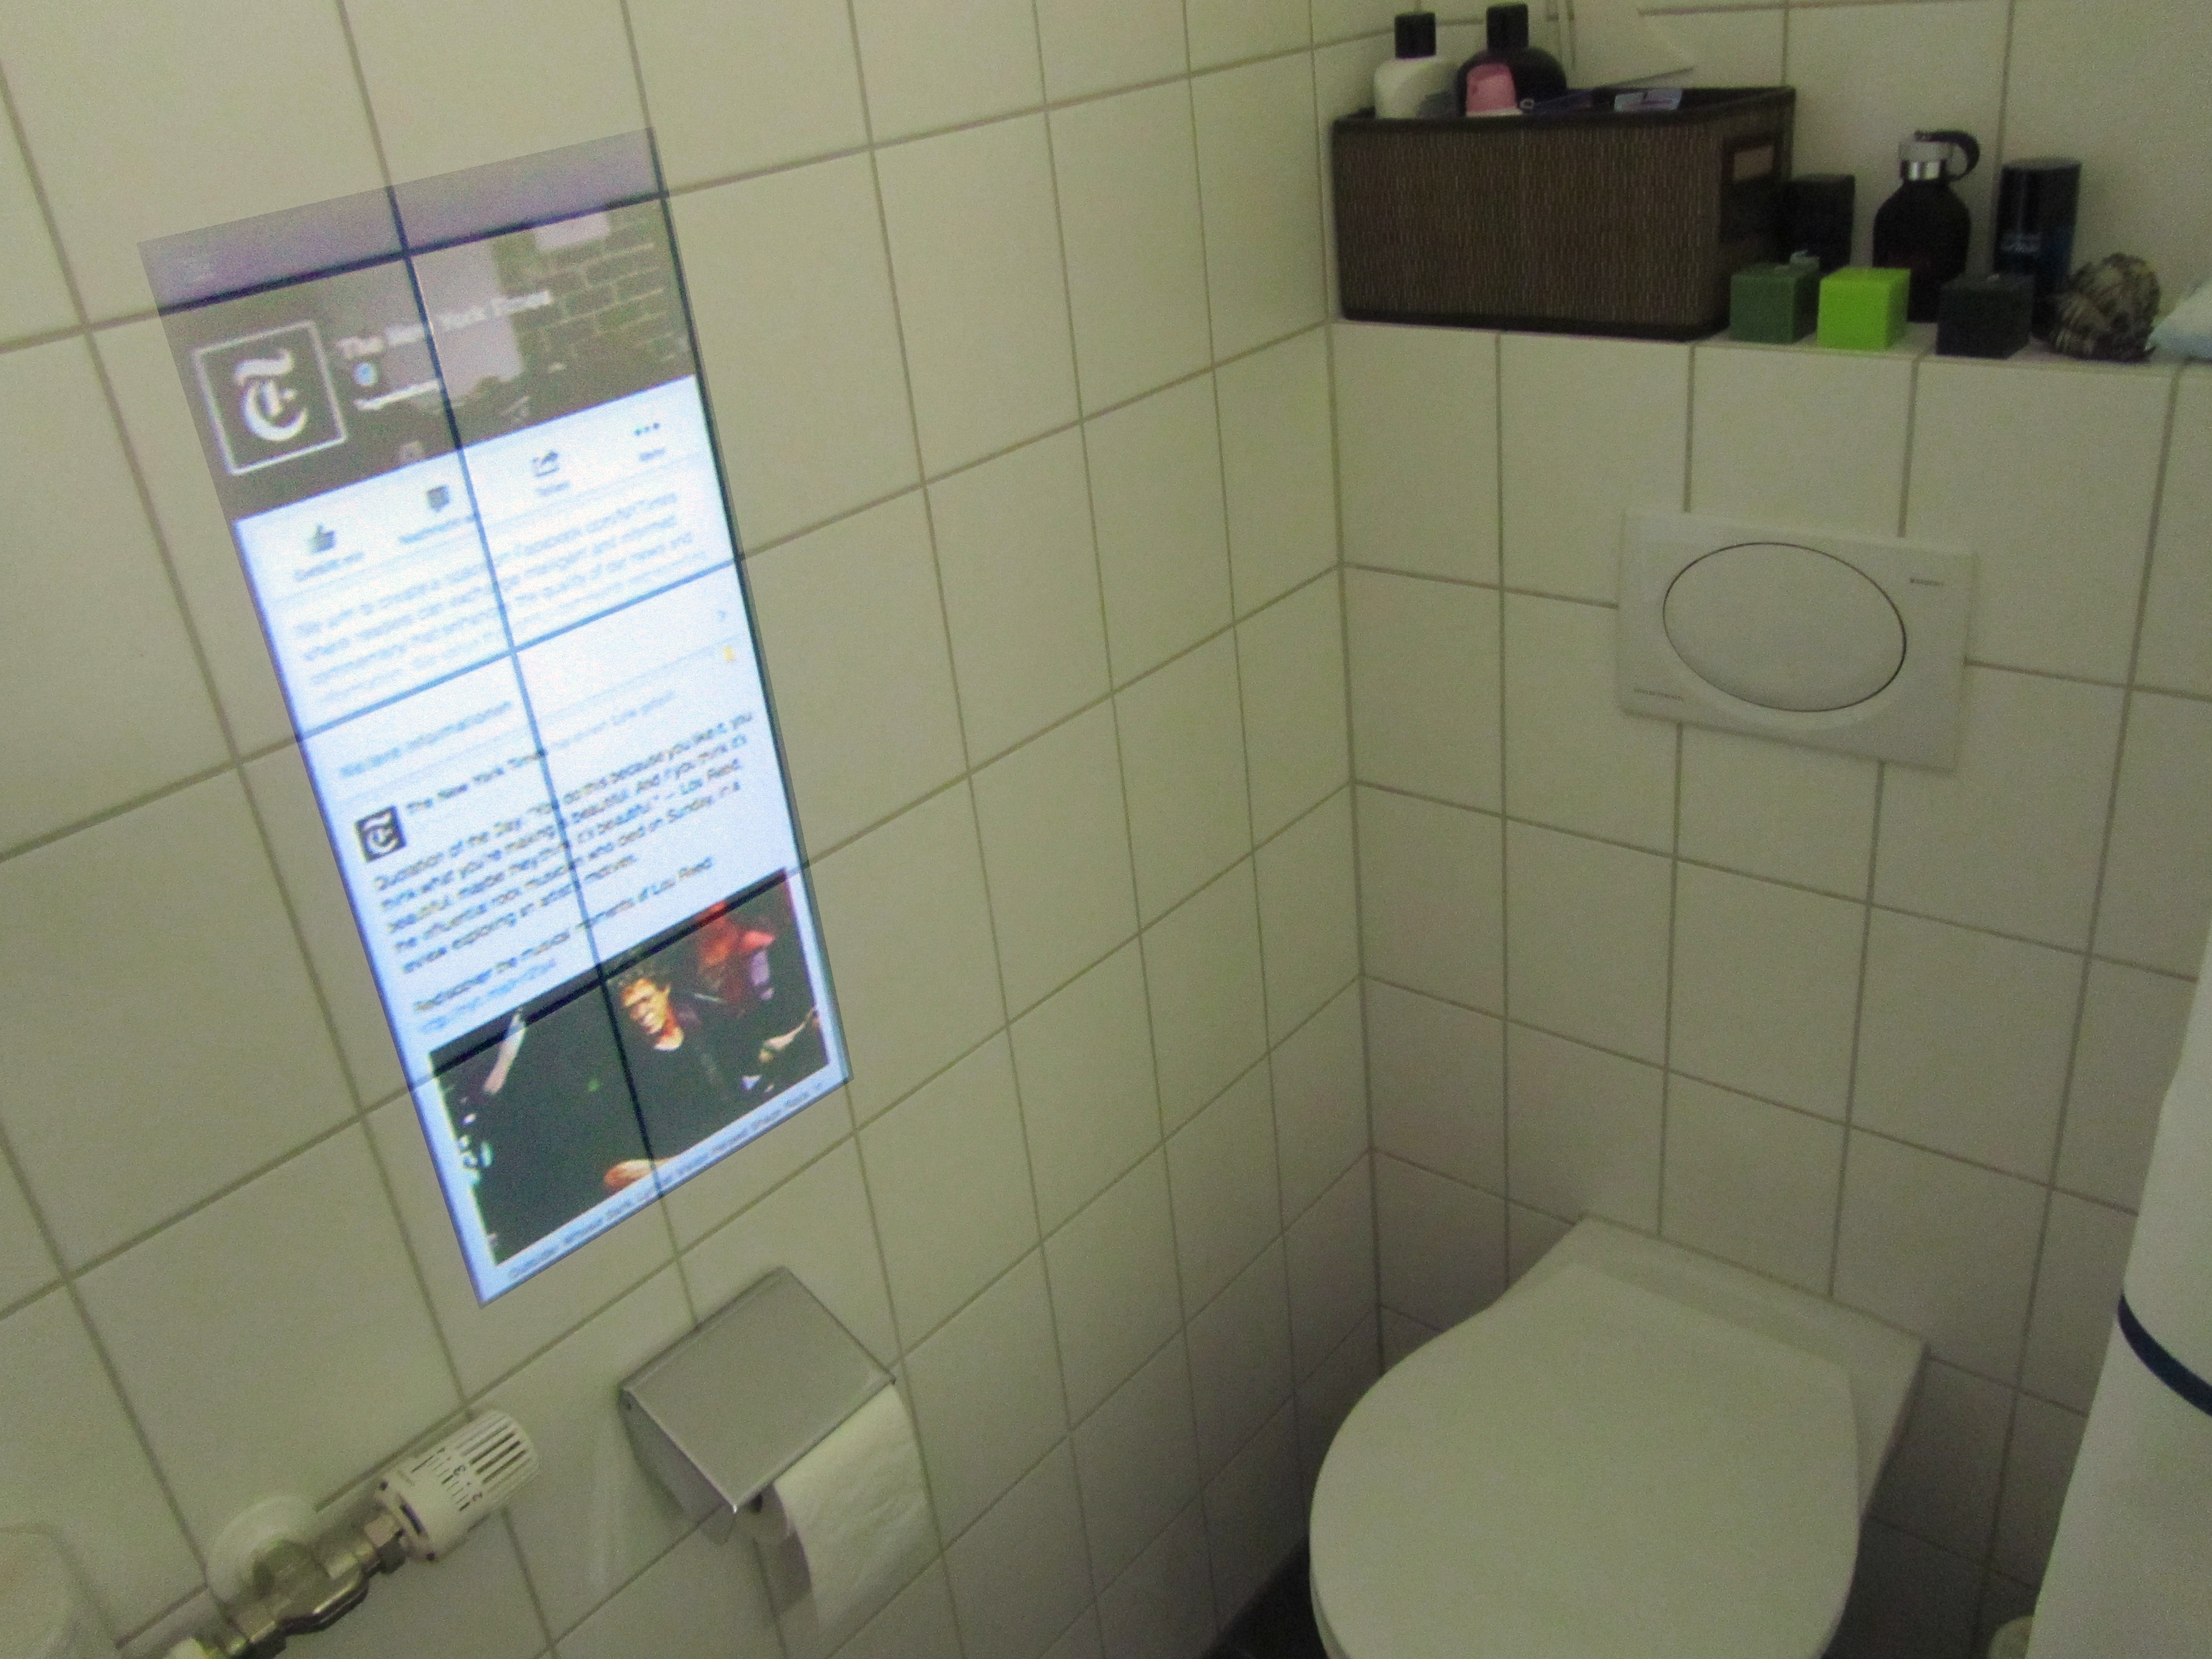
\includegraphics[width=\textwidth]{images/interview/bath02.jpg}
                \caption{Restroom setup}
                \label{img:bath01}
        \end{subfigure}
       \caption{Bath and restroom setup}\label{img:bath}
\end{figure}
In the corridor of the flats participants created \emph{interaction spaces} on free parts of the walls or the doors. One participant also created an \emph{interaction space} on the floor before his front-door to use his doormat as a \emph{surface}. 

\subsection{Placement}
While trying different setups participants always try to mount or place the PROCAMS above body height.
The \ac{PROCAMS} were typically mounted at the ceiling in the centre of the room. Apart from that it was placed on top of higher furniture as cupboards or shelfs. Participants achieved with this kind of placement to minimise the occlusions caused by their bodies when move around the room. 
Dependent on the room size and use case the distance between the \ac{PROCAMS} and the \emph{displays} were \SI{0.7}{\metre} to \SI{3.5}{\metre}. For example only \SI{0.7}{\metre} at the working desk and up to \SI{3.5}{\metre} in the living room when aligned to the large \emph{surface} on the opposite wall of the sofa.

\subsection{Widgets}
Over the course of the interviews, participants propose several widgets. In the kitchen, they describe a widget presenting a digital recipe book. A typical setup using cooking instructions in the kitchen is illustrated in~\autoref{img:cooking2}. 

Another widget which was mentioned several times, especially in the kitchen and working room is a widget which takes track of notes.
In the kitchen in particular a shopping list where items could easily be added and get synchronised with the smart phone was desired. 

Many participants motivate widgets which can be categorised into social media. Especially Facebook and Twitter or pre-configured feeds based on interests were mentioned. Besides social media, a widget presenting news or dynamic information was outlined. In particular global news, weather, sporting news, the TV guide, calendar or the bus timetable were listed. A news widget rendered at the dining table is depicted in~\autoref{fig:newsTable}. Such a widget should also appear, in the vicinity of the user after awaken, to inform him about the latest and upcoming events.

When the PROCAMS is not actively used participants had two ideas how to use the system in an alternative way. On the one hand, they suggested a widget which shows a simple clock or even a combination of different clocks for different time zones. The clock widget should also provide a timer and alarm function to support users while cooking or waking up. This use case is illustrated in~\autoref{img:clock}  On the other hand participants had the idea to use the PROCAMS as an ambient light source. The system could move slowly around and illuminate the room in desired fading colours.

\begin{figure}
        \centering
               \begin{subfigure}[b]{0.31\textwidth}
                \includegraphics[width=\textwidth]{images/interview/kitchen2.jpg}
                \caption{Cooking instruction setup}
                \label{img:cooking2}
        \end{subfigure}
\hfill
        \begin{subfigure}[b]{0.31\textwidth}
                \includegraphics[width=\textwidth]{images/interview/eat.jpg}
                \caption{News on dining table}
                \label{fig:newsTable}
        \end{subfigure}
        \hfill
        \begin{subfigure}[b]{0.31\textwidth}
                \includegraphics[width=\textwidth]{images/interview/kitchen1.jpg}
                \caption{Clock setup}
                \label{img:clock}
        \end{subfigure}
        \caption{Proposed setups and widgets}\label{fig:animals}
\end{figure}

Participants wanted to use the large \emph{surfaces} mainly for two reasons. First they want to replace the television or the media centre with a corresponding widget. Second, especially in the corridor, the \emph{surface} is used to render a digital image frame showing for example the latest holiday photos. In addition, some participant described an interactive music player which visualises the music on the large \emph{display} and presents a control widget in the vicinity of the user e.g. the sofa table. 

Focusing on the sofa table a widget for playing board games was described. Participants wished to combine a projected board with real tokens to play games with dynamic boards. 

Other stated ideas were for instance a digital whiteboard, a widget for action items and a reminder in the working room. Or, a remote control widget for all entertainment devices as a replacement for several different remotes they own.
Four participants also imagined using the \ac{PROCAMS} for home automation purposes or even as video door interphone. Another idea which was mentioned regarding the desk was a widget with shortcuts which could trigger events on the PC. For example, launching the mail application or control the music playback. An interesting last idea only named once, refers to the \emph{display} created at the doormat. A widget should appear there which shows, depending on a status, a away or welcome message.

\subsection{Interaction}
As interaction method participants brought up touch interaction in the first place. It appears to be most obvious interaction concept for interaction with widgets. Secondly they named voice interaction. Participants preferred voice interaction in the kitchen since they need their hands while cooking or they do not want to touch the surface because of dirty hands. Other known concepts mentioned were mid air gestures for scrolling or using a laser pointer to trigger buttons when they are not in the vicinity.

Two participants describe more unique interaction concepts. The first wants to use real physical objects to interact with a widget.  For example, they described a widget showing a counter which increases every time a coffee cup is placed on it. The other wanted to interact via the shadow they produces when the finger is in the light beam of the projector. In particular, this would be usable in some of the bedroom setups where the PROCAMS was close to the user.
Unfortunately, there were no extra novel interaction concepts elaborated. A possible reason could be the well known and daily used touch interaction.


\section{Findings}\label{sec:findings}
During setting up arrangements in the different rooms or final discussion, participants expressed several ideas or ask questions which lead to the following special explanatory notes. While elaborating setups in the bathroom, four participants remark privacy concerns due to the built-in camera. They claimed not to use a PROCAMS in this room. In addition, two participants stated in the bedroom to try to minimise the number of technical devices and therefore would not use a PROCAMS there.

To switch between different \emph{interaction spaces}, the \ac{PROCAMS} should be movable and listen to voice commands or switch to the \emph{surface} the user is tapping on. In total 67\% of the participants want a movable \ac{PROCAMS}. Eight of them propose a PROCAMS, which moves automatically. Four of them want to control by direct manipulation. Furthermore, five participants suggested a battery powered version of a \ac{PROCAMS}. The idea behind it was to enable the possibility to take the \ac{PROCAMS} to friends and share content on a large interactive \emph{display}. Additionally, some participants described the possibility to own only one or two \ac{PROCAMS}, many for financial reasons, which can seamlessly switch between rooms and always know the available \emph{surfaces} and related \emph{displays}. One participant described an intelligent wall plug which takes control of storing \emph{surfaces} for the specific position of the plug and also recharges the portable \ac{PROCAMS} submodule.

Another feature which was mentioned is multi user, multi \emph{display} support. A participant explained that they wanted to use a \emph{display} in a \emph{surface}, for example the kitchen table, while another person can interact with another \emph{display} hosted on the same \emph{surface}.
All participants agreed that the projected widgets need to be in in focus without any interaction. Furthermore, projections have to be light intensive to ensure visibility during daytime.  

For instantiating new \emph{displays} participants explained to use touch gestures or a smart phone as a remote. Further calibration and configuration tasks should not be forwarded to the user, participants said. 

Most participants (10) were satisfied with the dimensions and plain design of the mock-up. Most of the time the PROCAMS will be mounted at the ceiling and is thus not directly in the field of vision. However, some of the participants indicated that they prefer a lighter (3), more robust (1) or more aesthetic (2) version.

\section{Summary}
Interviews with 18 participants were conducted, thereby gaining some new and interesting use cases for a \ac{PROCAMS}. In particular, the wide variety of already existing things which \ac{PROCAMS} can replace is remarkable. Wall paintings, television, clocks, printed bus timetables, alarm clock or a remote control to cite just a few.

Noticeable is that all participants chose only flat \emph{surfaces} even after clarifying that it would be feasible to project without distortion to irregular surfaces. Participants created solutions to get the most of the \ac{PROCAMS} by proposing a movable and straightforward  mount and unmountable system.

On the negative side participants claim about privacy issues.  Some of them also mentioned that depending on the situation parts of the body could occlude larger parts of the display. The overall positive interviews with various ideas lead to some sufficient requirements. Aspiration of the resulting \ac{PROCAMS} is to be available to everyone in a domestic environment.